\section{Simulación: primera aproximación}
Como se ha mencionado en la introducción, el objetivo principal de este
proyecto es evitar accidentes que involucre \gls{vru}s en un escenario urbano.
Aunque la solución propuesta es completamente funcional, tan solo ha sido
probada a pequeña escala. Para intentar obtener el comportamiento que esta
solución tendría en escenarios más complejos, se ha decidido probar la
aplicación en un escenario simulado con más vehículos (4), más ciclistas (8),
y modelando los parámetros de comunicaciones; los cuales son críticos para la
fiabilidad de la aplicación.

\begin{figure}[h]
	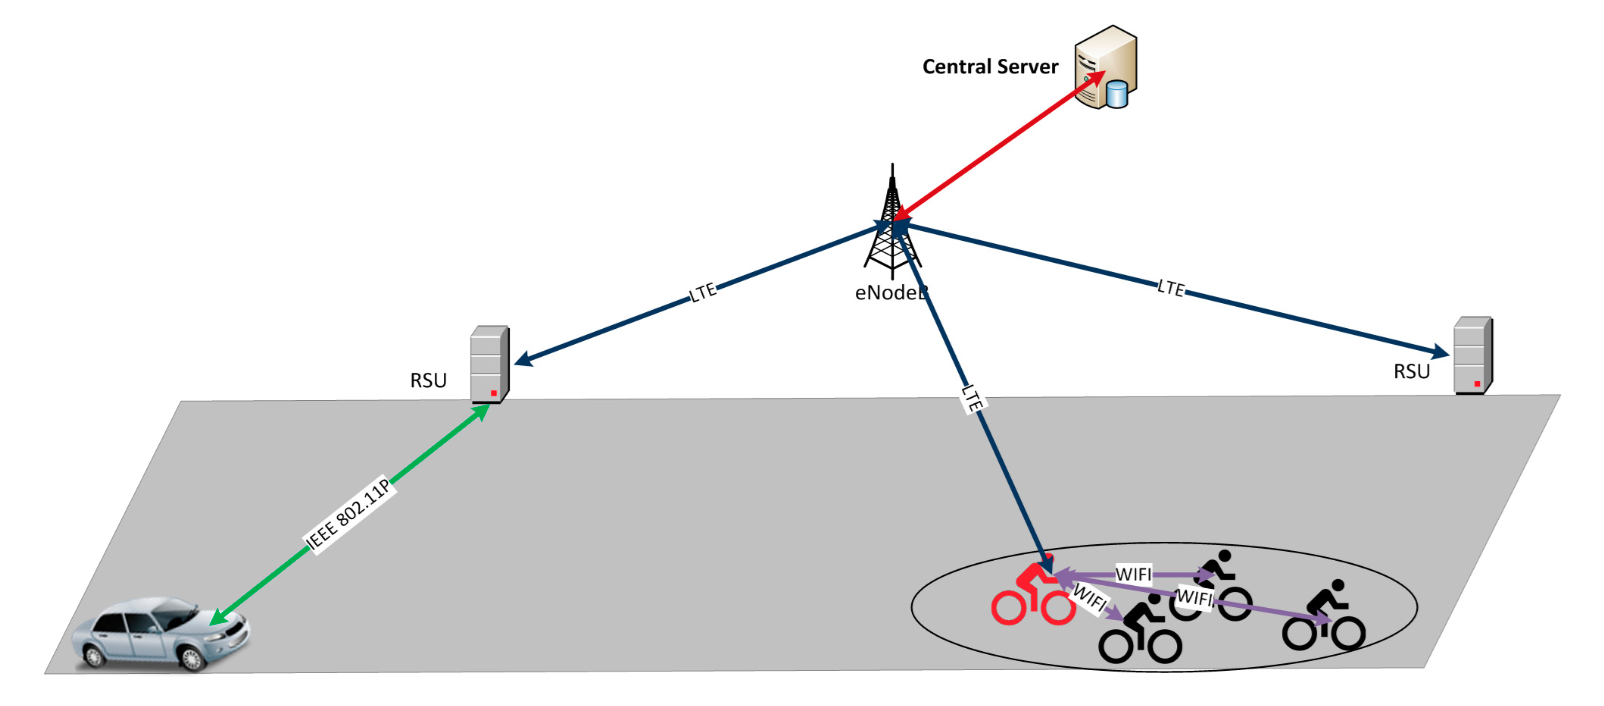
\includegraphics[scale=0.6]{simulacion-vehiculos}
	\caption{Descripción de la arquitectura simulada}
	\label{fig:simulacion-vehiculos}
\end{figure}

En la Figura \ref{fig:simulacion-vehiculos} se muestra la arquitectura diseñada
para validar el rendimiento de la solución en un sistema \gls{fcd} por medio de
una simulación. Esta arquitectura permite el intercambio de información entre
sensores móviles (obtenidos de vehículos y ciclistas) gracias a un servidor
central que tiene una visión global del escenario en carretera.

Esta variedad de tecnologías en la arquitectura permite la ejecución de tres
fases principales:

\begin{enumerate}
	\item Obtención de datos: esta fase consta de todo lo relacionado con enviar
	información al servidor central. Por lo tanto, por una parte, como todo
	vehículo actúa de sensor mandando \gls{cam}s, cada \gls{rsu} es capaz de
	conocer la información sobre la posición de todos los vehículos que se
	encuentran en su área de cobertura y retransmite esta información al
	servidor central. Por otra parte, las bicicletas también están enviando
	mensajes periódicos con la información sobre su posición dentro de una red
	Wi-Fi; por consiguiente, el líder de los ciclistas es capaz de reunir toda
	esta información sobre el grupo y enviarla al servidor central a través de
	tecnología \gls{lte}.

	\item Gestión de información centralizada: la recepción de información
	actualizada sobre la situación en carretera por el servidor central permite
	comprobar qué vehículos pueden encontrarse con un grupo de ciclistas e
	informar a las bicicletas sobre la posición de los vehículos.

	\item Dispersión de mensajes de alerta: esta fase está encargada de enviar
	información de los vehículos a los ciclistas, y la información de los
	ciclistas a los vehículos. Por consiguiente, el servidor central envía la
	información de los ciclistas al \gls{rsu} a través de \gls{lte}, y las
	\gls{rsu} dispersan esta información a través de de \gls{802.11p} con el
	objetivo de ser recibidos por los vehículos interesados en su área de
	cobertura. Al mismo tiempo, el servidor envía información sobre los vehículos
	que se aproximan al líder de ciclistas por medio de \gls{lte} y el líder de
	ciclistas dispersa esta información al resto de ciclistas a través de Wi-Fi.
\end{enumerate}

\subsection{Configuración de la simulación}
El objetivo principal de la simulación es mostrar la viabilidad y el
rendimiento de la arquitectura anteriormente propuesta. Por lo tanto, esta
arquitectura es evaluada empleando un simulador en red de eventos discretos
NS-3 \cite{14}, el cual es open source y validado por la comunidad de
investigación. Además, NS-3.21 provee de modelos para la asistencia de redes
vehiculares heterogéneas, incluyendo modelos de comunicaciones de corto alcance
como Wi-Fi y \gls{802.11p} y redes móviles como \gls{lte}. Para generar las
rutas que realizarán los vehículos y bicicletas durante la simulación NS-3,
se emplea el simulador de tráfico\gls{sumo} [15]. El escenario simulado es un
área suburbana de Bilbao donde hay normalmente hay múltiples grupos de
ciclistas y el flujo de vehículos es irregular. Los vehículos y bicicletas se
mueven durante 600 segundos en una carretera de 5 km. La Tabla
\ref{tab:parametros_simulacion} detalla los detalles de la simulación empleados
durante la evaluación.

\begin{table}[h]
	\centering
	\caption{Tipo de mensajes en grupo}\label{tab:parametros_simulacion}
	\begin{tabular}{lll}
		\toprule
		\textbf{Tipo} & \emph{Parámetro} & Valor \\
		\midrule
		Vehículos	&	Frecuencia \gls{cam}	&	1 Hz \\
		\gls{rsu}	&	Frecuencia de actualización TMC	&	Mensaje \gls{cam} recibido por el vehículo \\
		Bicicleta	&	Frecuencia de actualización del líder	&	1 Hz \\
		Bicicleta líder & Frecuencia de actualización TMC	& 1 Hz \\
		\midrule
		\multirow{5}{*}{Escenario}	&	Tipo	& Suburbano \\
													&	Número de vehículos	&	4	\\
													&	Número de ciclistas &	8	\\
													&	Velocidad del vehículo	&	10-70 km/h \\
													&	Velocidad del ciclista	&	25-30 km/h \\
		\midrule
		\multirow{5}{*}{Red IEEE 802.11p} &	Bit rate	&	3 Mbps \\
													&	Banda ancha	&	10 MHz \\
													&	Banda de frecuencia	&	5.9 GHz \\
													&	Potencia máxima de TX	&	21 dBm \\
													&	Modelo de propagación	&	Nakagami \\
		\midrule
		\multirow{5}{*}{Red IEEE 802.11b} &	Bit rate	&	1 Mbps \\
													&	Banda ancha	&	20 MHz \\
													&	Banda de frecuencia		&	2.4 GHz \\
													&	Potencia máxima de TX	&	16 dBm \\
													&	Modelo de propagación	&	Nakagami \\
		\bottomrule
	\end{tabular}
\end{table}

\subsection{Mediciones y resultados}
Las siguientes mediciones son considerados en este estudio:
\begin{itemize}
	\item Retraso en la recepción de los ciclistas (ms): el tiempo que ha pasado
	entre que el mensaje ha sido transmitido por el vehículo y la recepción del
	mensaje por el ciclista.

	\item Retraso en la recepción de los vehículos (ms): el tiempo que ha pasado
	entre que el mensaje ha sido transmitido por el líder ciclista y lo ha
	recibido el vehículo.
\end{itemize}

\begin{figure}[h]
	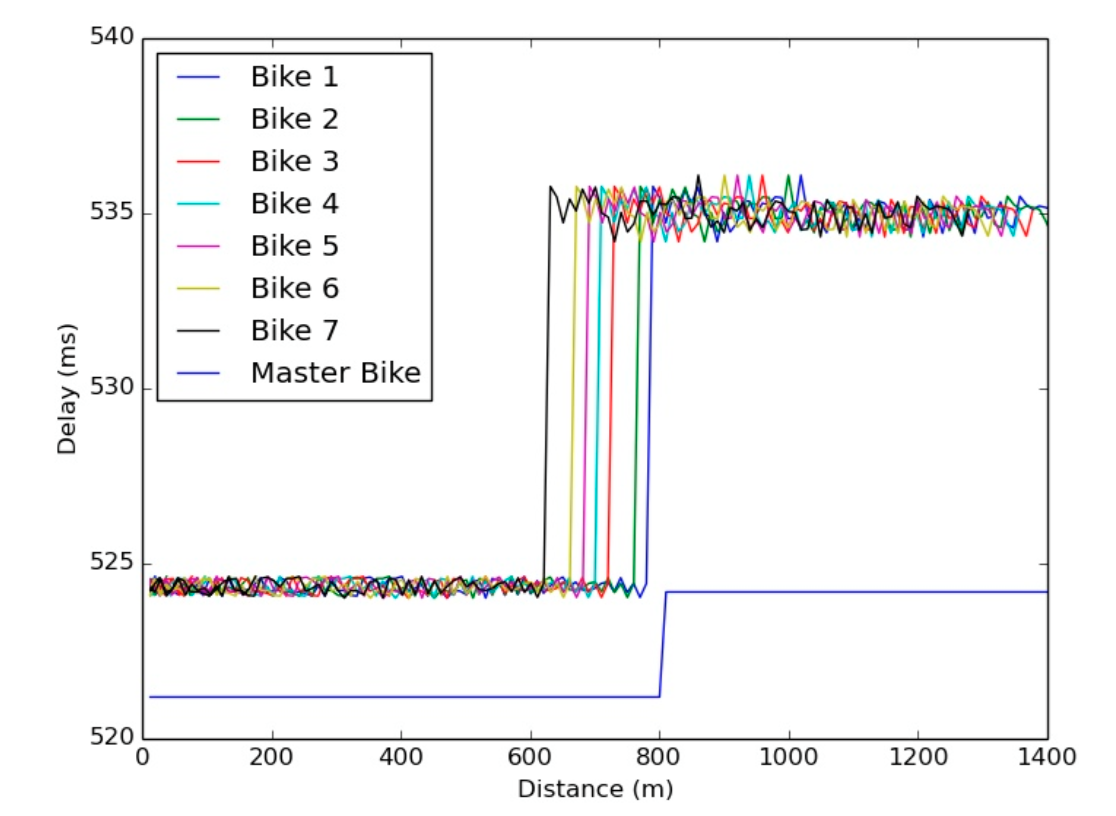
\includegraphics[scale=0.6]{delay-recepcion-ciclista}
	\caption{Retraso en recepción del ciclista}
	\label{fig:delay-recepcion-ciclista}
\end{figure}

\begin{figure}[h]
	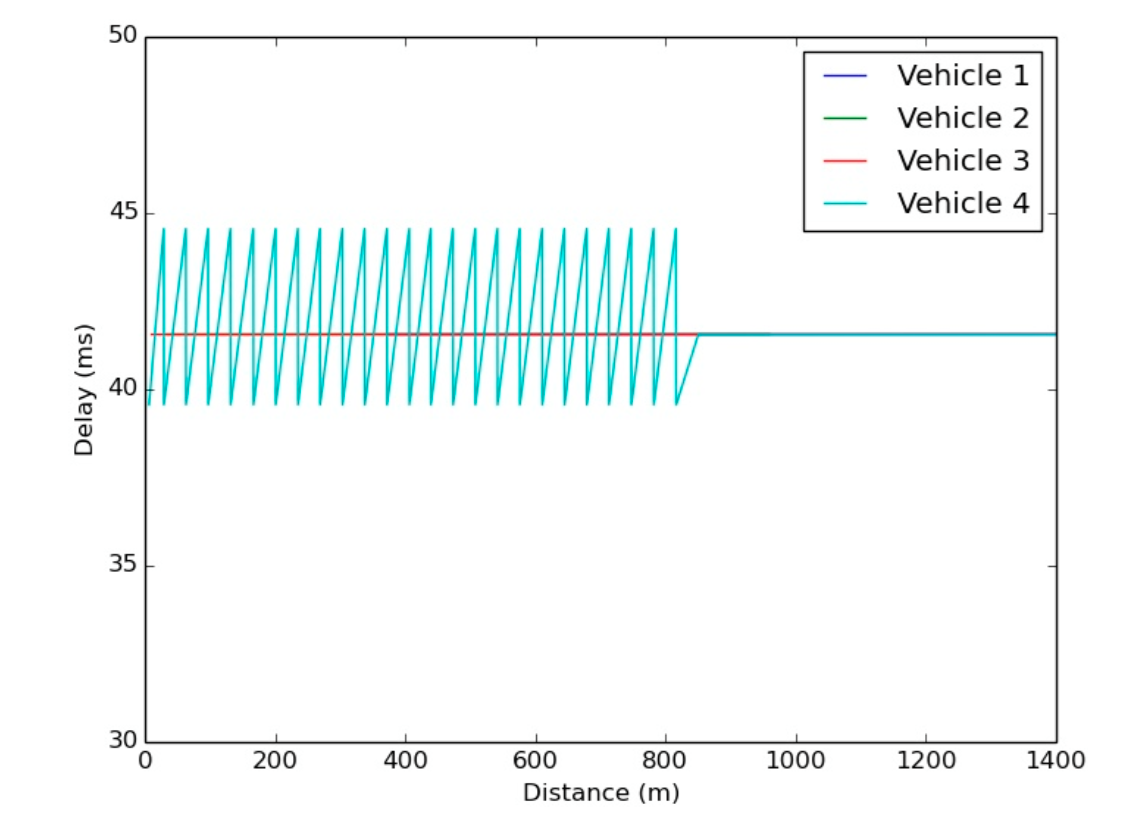
\includegraphics[scale=0.6]{delay-recepcion-vehiculo}
	\caption{Retraso en recepción del vehículo}
	\label{fig:delay-recepcion-vehiculo}
\end{figure}

La validación de los resultados de la simulación es necesaria para desplegar la
aplicación en entornos reales. La fiabilidad depende del retraso del mensaje de
alcanzar el destino. Por lo tanto, la Figura \ref{fig:delay-recepcion-ciclista}
muestra la media de retraso de un mensaje que sale de un vehículo a una
bicicleta dependiendo de la distancia entre el vehículo y la bicicleta. Como
se muestra en la figura \ref{fig:delay-recepcion-ciclista}, el tiempo que un
mensaje necesita para alcanzar al líder de la bicicleta es menor que el resto
de bicicletas porque el líder es el encargado de dispersar el mensaje del
vehículo al resto de bicicletas a través de la red Wi-Fi. La Figura
\ref{fig:delay-recepcion-vehiculo} muestra el retraso de recepción del vehículo,
que es casi constante para todas las distancias.

Comparando los resultados de las Figuras \ref{fig:delay-recepcion-ciclista} y
\ref{fig:delay-recepcion-vehiculo}, se puede observar que el retraso de
recepción de la bicicleta está en un rango de entre 522 ms y 535 ms, pero la
media de retraso de recepción de un vehículo es de 40 ms. Esta diferencia es
debida a la ruta que cada mensaje tiene que seguir y la frecuencia de
actualización del \gls{tmc} en el \gls{rsu} y líder de ciclistas.

El retraso de recepción en el ciclista está definido en la Ecuación
\ref{eq:delay_lider} para el líder de ciclistas y en la Ecuación
\ref{eq:delay_seguidores} para el resto de bicicletas en el grupo (seguidores):

\begin{equation}\label{eq:delay_lider}
D_{lider} = D_{v-RSU} + D_{RSU-TMC} + D_{TMC-BM}
\end{equation}

\begin{equation}\label{eq:delay_seguidores}
D_{seguidores} = D_{v-RSU} + D_{RSU-TMC} + D_{TMC-BM} + D_{BM-B}
\end{equation}
donde
\begin{itemize}
	\item $D_{v-RSU}$ es el tiempo desde que el mensaje ha sido generado en el
	vehículo hasta que el \gls{rsu} recibe dicho mensaje.

	\item $D_{RSU-TMC}$ es el tiempo que pasa desde que el \gls{rsu} recibe el
	mensaje desde el vehículo hasta que es recibido por el \gls{tmc}.

	\item $D_{TMC-BM}$ es el tiempo que pasa desde que el \gls{tmc} recibe el
	mensaje desde la \gls{rsu} hasta que es recibido por el líder.

	\item $D_{BM-B}$ es el tiempo que pasa desde que el líder recibe el mensaje
	del \gls{tmc} hasta que es recibido por los ciclistas que están en la red
	Wi-Fi.
\end{itemize}

El retraso de la recepción por el vehículo está definida por la Ecuación
\ref{eq:delay_vehiculo}:
\begin{equation}\label{eq:delay_vehiculo}
D_{vehículo} = D_{BM-TMC} + D_{TMC-RSU} + D_{RSU_V}
\end{equation}
donde
\begin{itemize}
	\item $D_{BM-TMC}$ es el tiempo que pasa desde que el mensaje es generado en
	el líder de ciclistas hasta que es recibido por el \gls{tmc}.

	\item $D_{TMC-RSU}$ es el tiempo que pasa desde que el mensaje es recibido
	por el \gls{tmc}, enviado por el líder de ciclistas, hasta que es recibido
	por el \gls{rsu}.

	\item $D_{RSU-V}$ es el tiempo que pasa desde que el \gls{rsu} recibe el
	mensaje procedente del \gls{tmc}, y es recibido por el vehículo.
\end{itemize}

La diferencia viene dada porque el \gls{tmc} solo envía mensajes de alerta las
\gls{rsu}s y al líder de ciclistas cuando recibe un mensaje de un vehículo.
Como el grupo de ciclistas está actualizando la información del \gls{tmc} a
través del líder de ciclistas a una frecuencia de 1 Hz, como se muestra en la
Figura \ref{fig:simulacion-diagrama-secuencia}, hay un retraso desde que el
\gls{rsu} recibe un mensaje desde el vehículo hasta que lo retransmite al
\gls{tmc}. Sin embargo, este retraso no existe desde el líder de ciclistas
hasta el \gls{tmc} ya que el líder de ciclistas está generando un nuevo mensaje
con la información del grupo de ciclistas.

\begin{figure}[h]
	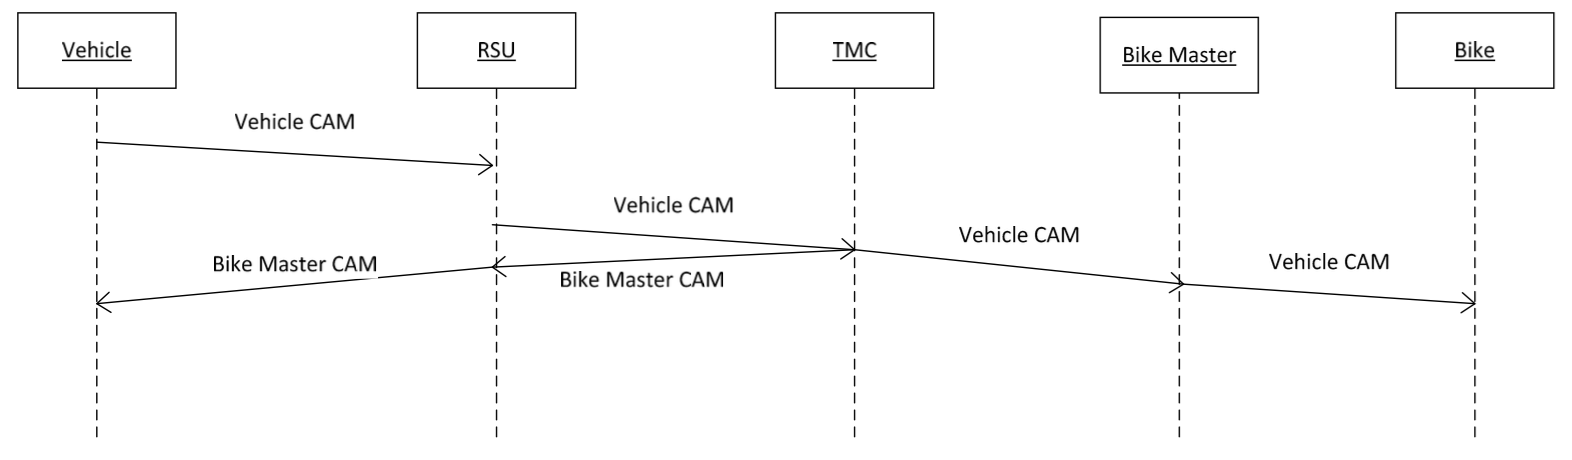
\includegraphics[scale=0.6]{simulacion-diagrama-secuencia}
	\caption{Diagrama de secuencia del sistema}
	\label{fig:simulacion-diagrama-secuencia}
\end{figure}
